%%%%
\section{Black Carbon (BC)}

Medidas de BC podem ser realizadas de forma absoluta ou relativa, sendo a 
segunda incomparavelmente mais simples e de menor custo que a primeira. 
No caso de medidas relativas por refletância pode-se usar os mesmos filtros 
da análise elementar por XRF-ED (PTFE ou policarbonato), pois ambas técnicas são 
não destrutivas. Todas operações envolvidas nas medições por refletância 
consomem algo em torno de um a dois minuto, em média, possibilitando a 
determinação de centenas de amostras em poucos dias.

Aetalômetro é outra medida relativa de BC, mais antiga que refletância,
onde um feixe colimado de luz monocromática é incidido sobre o
filtro com amostra coletada medindo-se a quantidade luz absorvida via 
atenuação. Medidas relativas de BC são realizadas desde 1980 e ainda hoje são 
intensamente empregadas \citep{targino2016}.

Thermal Optical-Reflectance (TOR) ou 
Thermal-Optical Transmittance (TOT), fornecem medidas absolutas de BC e OC
(Carbono Orgânico), mas são destrutivas e necessitam de um filtro especial e 
de um aparato de medidas exclusivo, tendo custo bem mais elevado.

%%%%
\subsection{Refletância}

Concentrações de BC foram obtidas por refletômetro do tipo 
\textit{Smoke Stain Reflectometer} modelo EEL43D da empresa Diffusion System.
Devido à sua simplicidade, é tradicionalmente usado para medidas de BC em 
amostras ambientais \citep{lack2014}. 

A técnica baseia-se na alta seção de choque de absorção de luz pelo BC, 
na região do visível, e é assumido que não existem outras 
partículas absorvendo a luz incidente que não as de BC, sendo considerada 
uma técnica de medida de BC relativa, pois não mede diretamente o BC. 

\begin{figure}[H]
  \centering
  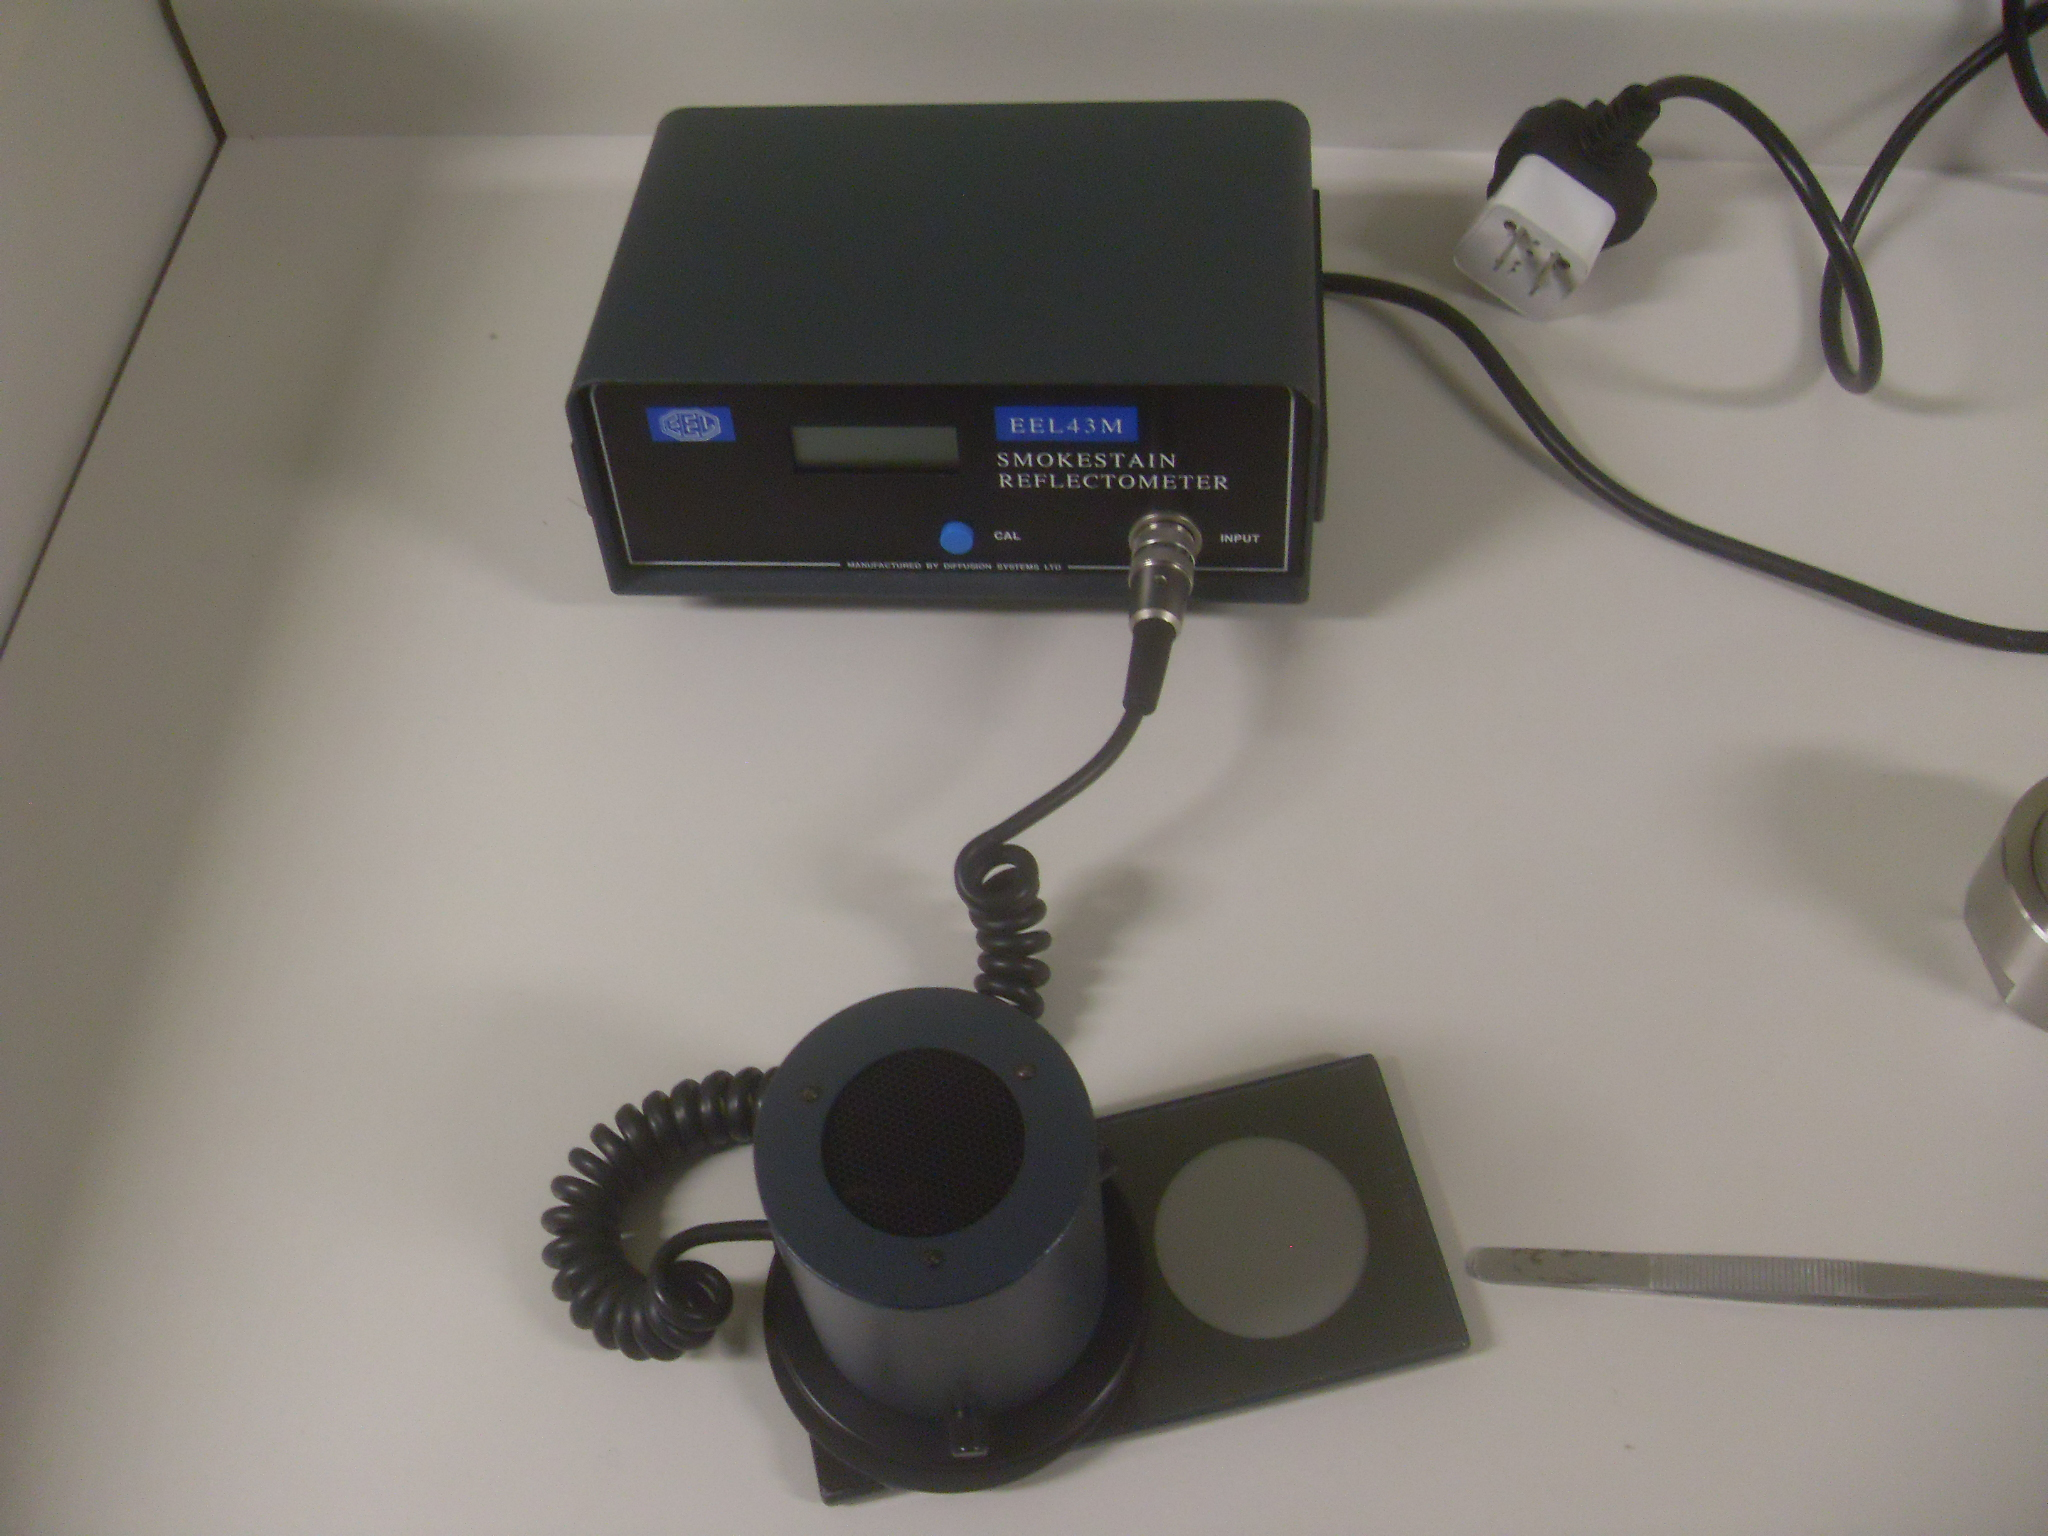
\includegraphics[width=0.5\textwidth]{../inputs/images/refletometro.jpg}
  \caption{Refletômetro Diffusion System modelo ELL43D 
           e peças auxiliares de fixação LAPAt}
\end{figure}

Na refletância, uma área definida da amostra é ilumindada por lâmpada de 
tungsténio. Parte da luz difusora incidente é absorvida pelas partículas
do filtro e parte refletida. Uma fotocélula com orifício circular, localizada
entre a lâmpada e a amostra, mede a porcentagem da luz refletida (I).
Um filtro branco é usado para fixar o 100\% das leituras a cada 3 medidas.

A absorção de luz que atravessa um meio com coeficiente de absorção ($\alpha$) 
homogêneo, segue um processo clássico. A intensidade I da luz em um ponto x da
amostra (meio) homogênea, decai $-dI$ ao atravessar uma espessura $dx$, 
sendo o decaimento diretamente proporcional a I:

\begin{equation}
  \label{eq:dIdx}
   \frac{dI}{dx} = -\alpha I
\end{equation}

fazendo-se a separação das variáveis, pode-se integrar os dois lados da equação:

\begin{equation}
  \int_{I_0}^{I} \frac{dI}{I} = - \int_{0}^{D} \alpha dx
\end{equation}

Resultando em uma relação exponencial entre o decaimento da intensidade do feixe
de luz incidente ($I_0$) e a intensidade transmitida ($I$), 
em função da espessura (D) da amostra:

\begin{equation}
  \label{eq:I_BC}
  I = I_0 \cdot exp(-\alpha D)
\end{equation}

No caso da refletância o feixe de luz vai e volta pela amostra, ficando:

\begin{equation}
\label{eq:I_BC2}
  I = I_0 \cdot exp(-\alpha 2D)
\end{equation}

O detector opera sobre uma área fixa e, assim, a medida que nos interessa é a 
massa por unidade de área (A). Ao ser multiplicada pela área total de amostragem
no filtro ela nos dá a massa total coletada. A massa $m$ que o detetor observa é
$m = \rho.V = \rho.D.A$, onde $\rho$ é a densidade da amostra. 
Podemos usar esta relação para substituir $D$ na equação \ref{eq:I_BC2}, 
ficando:

\begin{equation}
  \label{m/a}
  I = I_0 \cdot exp \left( -\frac{2\alpha}{\rho}.\frac{m}{A} \right)
\end{equation}

Aplicando-se log nesta equação e rearranjando os termos, obtemos:

\begin{equation}
  \label{m/a_2}
  \frac{m}{A} = K(2-logI) 
\end{equation}


onde $\frac{1}{K} = 2.\frac{\alpha}{\rho}.log(e)$
é uma constante e usou-se que $I_0$=100\%, sendo log100 = 2.

Essa relação linear entre $\frac{m}{A}$ e log($I$) oferece bom ajuste empírico 
quando se trabalha com BC, permitindo a calibração do equipamento. 
Ressalve-se haver uma perda de linearidade para valores muito baixos de 
refletância (amostras muito carregadas).  

%%%%
\subsection{Thermal Optical Transmittance (TOT)}

Apresenta-se apenas os fundamentos gerais do TOT, pois o empregamos apenas para
calibrar o método de refletância. As medidas de TOT foram realizadas por outros
integrantes do projeto geral de pesquisa.
O TOT é um método absoluto para medir carbono orgânico (OC) e 
carbono elementar (EC). 
Baseia-se no fato que OC e EC convertem-se para gás em diferentes temperaturas 
e condições de oxidação \citep{birch1998}.

Aquecendo-se a amostra paulatinamente em ambiente não oxidante (presença de He),
ocorre progressiva volatização dos compostos orgânicos nas temperaturas mais 
baixas. A evaporação do carbono elementar ocorre acima de 580 $\degree C$.
Durante a fase de volatilização do OC, parte dele sofre pirólise, 
convertendo-se em EC e aumentando a concentração deste componente na amostra. 
Um sistema ótico com feixe de laser de intensidade controlada, registra este 
acúmulo em função da perda de transmitância da amostra.
Na fase de volatização do EC, contabiliza-se como OC, todo o EC extraído da 
amostra até o ponto em que o sistema óptico indique ter sido retomada a sua 
transmitância original. Daí em diante é que se passa a contabilizar o EC 
originalmente presente na amostra.
Faz-se a medida do C, oxidando-o para $CO_2$ ao passar por uma placa de dióxido
de magnésio aquecida, que segue por um catalizador de níquel, 
onde o dióxido de carbono é reduzido a metano $CH_4$. O $CH_4$ é quantificado 
com uma detector do tipo Flame Ionization Detector.
Para análises TOT é necessário fazer a coleta em filtros de quartzo, aumentando 
os custos e tornando mais complexa a logística das medidas, 
pois é necessário montar ponto de medida paralelos.
